\documentclass[10pt,a4paper]{article}

\usepackage[utf8x]{inputenc}
\usepackage[english]{babel}
\usepackage[T1]{fontenc,url}
\usepackage[hang,small,bf]{caption}
\usepackage{relsize}
\usepackage{setspace}
\usepackage{parskip}
\usepackage{lmodern}
\usepackage{microtype}
\usepackage{verbatim}
\usepackage{amsmath, amssymb, amsthm}
\usepackage{mathtools}
\usepackage{tikz}
\usepackage{physics}
\usepackage{algorithm}
\usepackage{algpseudocode}
\usepackage{listings}
\usepackage{enumerate}
\usepackage{graphicx}
\usepackage{float}
\usepackage{hyperref}
\usepackage{varioref}
\usepackage{siunitx}
\usepackage{todonotes}
\usepackage{color}
\usepackage[margin=3cm]{geometry}
\labelformat{equation}{equation~(#1)}
\labelformat{figure}{figure~(#1)}
\renewcommand{\exp}{\mathrm{e}^}
\newcommand{\halflife}{t_{\frac{1}{2}}}
\newcommand{\half}{\frac{1}{2}}
\newcommand{\planck}{$h = \SI{6.626e-34}{J.s}$}

\definecolor{light_green}{rgb}{0, 0.6, 0}
\definecolor{light_grey}{rgb}{0.5, 0.5, 0.5}
\definecolor{magenta}{rgb}{0.7, 0, 0.5}


\lstdefinestyle{py}{
    language = python,
    frame = single,
    showstringspaces = false,
    basicstyle = \small\ttfamily,
    breaklines = true,
    commentstyle = \color{light_grey},
    keywordstyle = \color{magenta},
    stringstyle = \color{light_green},
}


\begin{document}
\section*{Exercise 3.1 - Radioactive function}
\addcontentsline{toc}{section}{Exercise 3.1 - Radioactive function - \texttt{radioactive\_function.py}}
Implement the formula for radioactive decay from exercise 1.3 as a function, \texttt{N(N0, tau, t)}.

Write a test function that uses the values $N_0=\SI{4.5}{kg}$, $\tau=\SI{1760}{s}$, $t=\SI{600}{s}$, and confirms that you get the same results (within a tolerance) as you did with the carbon-11 in exercise 1.3 or 2.3. (This was approximately $\SI{3.2}{kg}$).

Don't set your tolerance smaller than $~10^{-4}$, because the answer you are comparing to is not entirely exact.


Filename: \texttt{radioactive\_function.py}




\section*{Exercise 3.2 - Quantum function}
\addcontentsline{toc}{section}{Exercise 3.2 - Quantum function - \texttt{quantum\_function.py}}

In exercise 2.5 we saw that particles trapped in a very small box of length $L$ are only allowed to have energies
\[	E_n = \frac{n^2 h^2}{8 m L^2}, \ \ \ \ n = 1,2,3\dots
\]
with $m$ being the particle's mass, and $h$ being Planck's constant $h = \SI{6.626e-34}{J.s}$

Write a function \texttt{quantum\_energy}, which takes two energy-levels\footnote{To specify: The function should take the index of the energy levels, $n$}, the length of the box, and the particle's mass as arguments, and returns the energy difference between the two energy levels.

Filename: \texttt{quantum\_function.py}



\section*{Exercise 3.3 - Wooden block}
\addcontentsline{toc}{section}{Exercise 3.3 - Wooden block - \texttt{block\_frictions.py}}
	In this exercise, you are supposed to create a program which finds out how far a wooden block with initial velocity $v_0\,$m/s will slide across surfaces of different materials. The material of the surface will affect the frictional force acting on the wooden block. 
	
	The position of the block can be expressed as such:
	\[
		x(t) = v_0t - \frac{1}{2}\mu g t^2
	\]
	where $\mu$ is a coefficient of friction and $g = 9.81\;\mathrm{m/s^2}$.
	
	One can find by some calculations at which time $T$ the block will stop moving. The time $T$ is found to be
	\[
	T = \frac{v_0}{\mu g}
	\]
	
	Define a function which takes a list of different coefficients of friction as parameter, calculates the position at time $T$, that is $x(T)$, and then stores the results in a list. The list of the calculated positions must then be returned by the function. 
		
		Let $v_0 = 5\,$m/s and the list of coefficients of friction be \texttt{[0.62, 0.3, 0.45, 0.2]}. Call the function and write out every position along with corresponding coefficient of friction.
	
	Filename: \texttt{block\_frictions.py}

	
	\section*{Exercise 3.4 - Hit target}
\addcontentsline{toc}{section}{Exercise 3.4 - Hit target - \texttt{hit\_target.py}}
	We will now simulate a game based on a simple physical model. 
	In this game a person is supposed to throw a ball at a wall with a target painted on. The person gets points according to where the ball hits at the wall.
	\begin{center}
	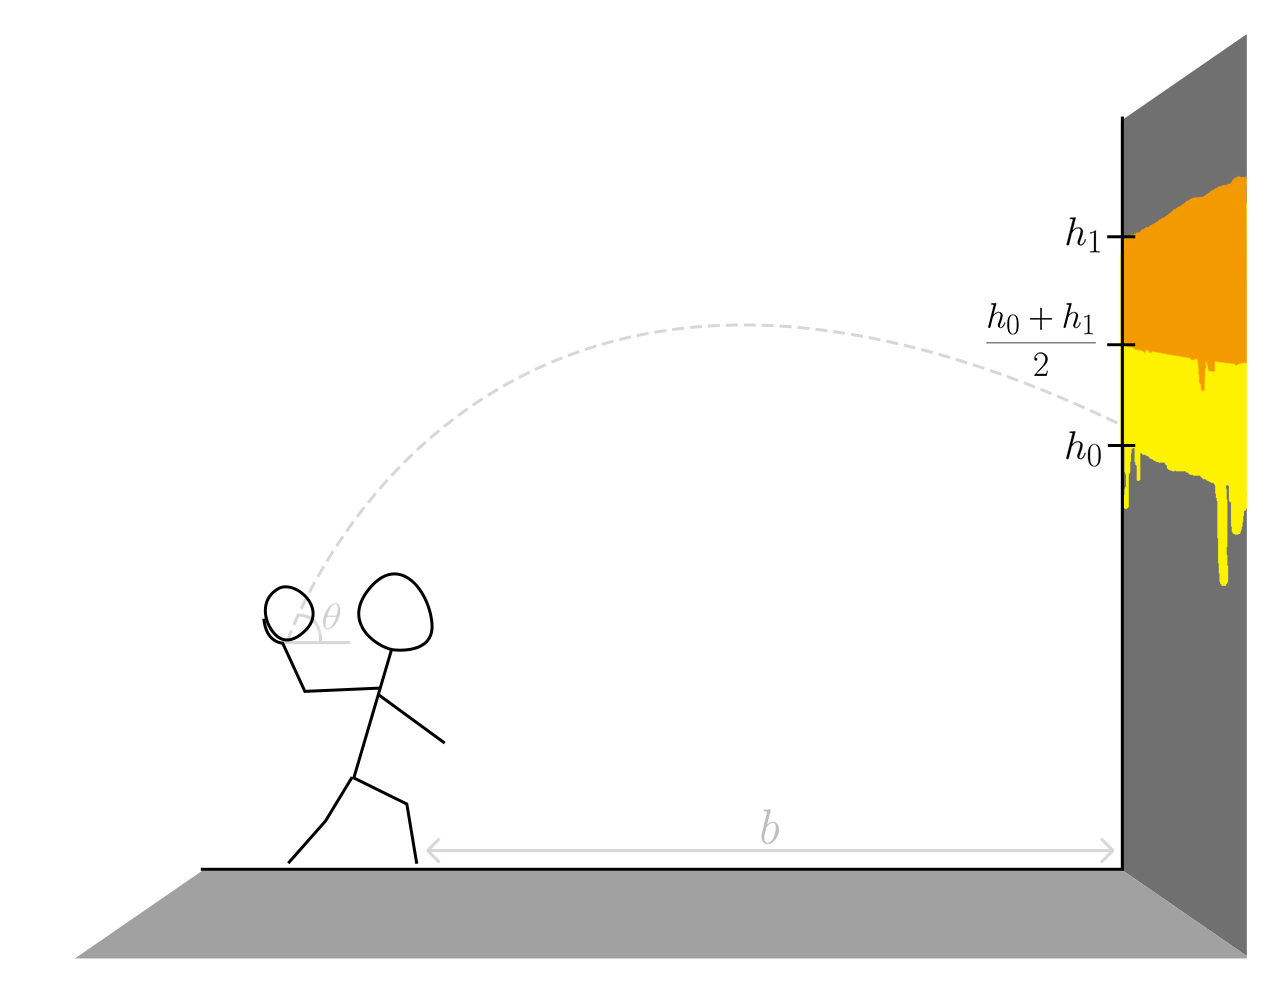
\includegraphics{fig_tegning_33-cp1.png}
	\captionof{figure}{Illustration of the system which we will base our game simulation on.}
	\end{center}

	The height of the ball can be modeled as:
	\begin{align*}
		y(t) &= -\frac{1}{2}g t^2 + v_0t\sin\theta
	\end{align*}
	where $v_0$ is the speed the ball has been thrown with, $\theta$ is the angle at which the ball has been thrown from and $g = 9.81\, \mathrm{m/s^2}$.
	
	\subsection*{a)}
	Write a function which returns the height of the ball at a given time $t$. 
	\subsection*{b)}
	
	One can find in our model that the ball will hit the wall at the time $T = \dfrac{b }{v_0\cos\theta}$ where $b$ is the distance between the person and the wall.  
	
	We must look at the value of $y(T)$ to be able to decide how many points the person will receive. The number of points must be calculated and returned from a function which you have to write.
	
	The target is painted such that it covers the wall between height $h_0$ and height $h_1$ where $h_0 < h_1$. The points are given according to the following rules: 
	\vspace{.2cm}
	\begin{itemize}
		\item The person gets 0 points if $y(T) < h_0 \text{ or } y(T) > h_1$
		\item The person gets 1 point if  $h_0 \leq y(T) <\frac{1}{2}(h_1 + h_0)$
		\item The person gets 2 points if $\frac{1}{2}(h_1 + h_0) \leq y(T) \leq h_1$
	\end{itemize} 
	\vspace{.2cm}
	
	Write a program which prints in a for loop how many points the person gets using your newly written function if $h_0 = 3\,\si{\meter}$, $h_1 = 3.5\,\si{\meter}$, $\theta = \dfrac{\pi}{4}$, $b = 3.5\,\si{\meter}$ for $v_0 = 15,16,19,22\,\si{\meter.\per\second}$.
	
	Filename: \texttt{hit\_target.py}


\section*{Exercise 3.5 - Downward cliff throw}
\addcontentsline{toc}{section}{Exercise 3.5 - Downward cliff throw - \texttt{cliff\_throw.py}}

\subsection*{a)}
We throw a rock straight down from a cliff, in a linear movement with constant acceleration. We ignore air resistance, and work only in one dimension. The velocity of the rock can be described either as a function of the distance it has traveled, $x$, or as a function of the time that has passed, $t$.
\begin{align}
v(t) &= v_0 + at\\
v(x) &= \sqrt{v_0^2 + 2ax}
\end{align}

(The latter one is often written $v^2-v_0^2 = 2ax$)

Where $v_0$ is the rock's initial velocity at $t=0$, and $a$ is its acceleration, which on earth is $a = \SI{9.81}{m/s^2}$. We pick downwards as our positive direction, meaning that $v_0$, $a$ and $x$ are always positive values.

Write two functions, \texttt{velocity1} and \texttt{velocity2}, based on the two equations above, which both returns the velocity of the rock from their three variables.


\subsection*{b)}
Write a test function \texttt{test\_velocity()}, which confirms that both functions returns the same velocity at a given time $t$ with the same initial velocity $v_0$. You can find the distance the ball has traveled at a given time from the formula
\begin{align*}
x(t) = v_0t + \half a t^2
\end{align*}


\subsection*{c)}
Expand \texttt{velocity1} from exercise a), such that $t$ also can be a list of time-points, in which case the function will return a list of velocities corresponding to those time-points. Note that the functions should still be capable of taking in $t$ as a single number, in which case the functions should also only return a single number.

\textbf{Hint:} Use an if/else block to check the type of $t$, and handle the two cases separately. Remember that the 'single number' might be either a float or integer.

Filename: \texttt{cliff\_throw.py}




\section*{Exercise 3.6 - Another wooden block}
\addcontentsline{toc}{section}{Exercise 3.6 - Another wooden block - \texttt{block\_frictions2.py}}
	We want to create a program which finds out how far a wooden block with initial velocity $v_0\,$m/s will slide across surfaces of different materials. The material of the surface will affect the frictional force acting on the wooden block. 
	
	The velocity and the distance of the wooden block at a time $t$ can be expressed as:
\begin{align*}
v(t) &= v_0 -  \mu g t \\
x(t) &= v_0t - \frac{1}{2}\mu g t^2
\end{align*}
where $\mu$ is a coefficient of friction and $v_0$ is the velocity of the block at time $t = 0$. 

\subsection*{a)}
Define a function which returns the distance $x(T)$ and takes $t$, $v_0$ and a coefficient of friction $\mu$ as parameter. 

\subsection*{b)}

Define a function which takes in a list of different coefficients of friction and returns a list of how far the block has moved for each of coefficient of friction. 

To do so, the function must also take $\Delta t$ as parameter, which is the time step we will use to find the velocity of the block. 

The function must then use a while loop to test for which time $t$ the velocity $v(t)$ becomes less or equal to 0. Use the time $t$ which has been found to calculate the distance $x(t)$. The distance must then be stored in a list. Let the function return the list when all of the distances has been calculated and stored. 

Let $v_0 = 5\,$m/s, $\Delta t = 0.0001\,$s and the list of coefficients of friction be \texttt{[0.62, 0.3, 0.45, 0.2]}.
\subsection*{c)}
Define a test function which tests if the list from b) are equal to the analytical distance $x\qty(\frac{v_0}{\mu g})$ at time $t = \frac{v_0}{\mu g}$ (this is the calculated time each block will use) for every coefficient of friction $\mu$. A suitable threshold to use when testing for equality between the calculated and analytical values is $10^{-7}$ in this task. 

Call the test function to test if you have gotten results which are more or less equal to the analytical distance for every $\mu$.  

Filename: \texttt{block\_frictions2.py}

\end{document}
